\label{ch:stand-van-zaken}
\graphicspath{{./img/}}
% Tip: Begin elk hoofdstuk met een paragraaf inleiding die beschrijft hoe
% dit hoofdstuk past binnen het geheel van de bachelorproef. Geef in het
% bijzonder aan wat de link is met het vorige en volgende hoofdstuk.

% Pas na deze inleidende paragraaf komt de eerste sectiehoofding.
\chapter{Stand van zaken}
\textbf{Inleiding}

In dit hoofdstuk wordt de huidige toestand van monolithische en microservice-architectuur besproken. De focus ligt hoofdzakelijk op het deel van microservices omdat de eindtoestand van de transformatie voor dit onderzoek het belangrijkst is.

\section{Microservice-architectuur}

\subsection{Service oriented architecture}
De term Service oriented architecture of SOA wordt vaak vermeld tijdens het bespreken van microservices. De twee architecturen hebben heel wat gemeenschappelijk maar er zijn toch wat verschillen. Daarom wordt er eerst uit geklaard wat deze verschillen zijn en welke aspecten de architecturen delen. 

SOA definieert een manier om softwarecomponenten herbruikbaar te maken via service-interfaces. Deze interfaces maken gebruik van gemeenschappelijke communicatiestandaarden. Hierdoor is het mogelijk om de services snel op te nemen in nieuwe applicaties zonder elke keer een zware integratie uit te voeren.

Iedere service vertegenwoordigt een business gerelateerd aspect. De service bevat de code en de nodige gegevensintegraties om het functionele aspect volledig en zelfstandig uit te voeren. Bijvoorbeeld het afhandelen van een betaling.\\

\begin{figure}
    \caption{Microservices}
    \centering
    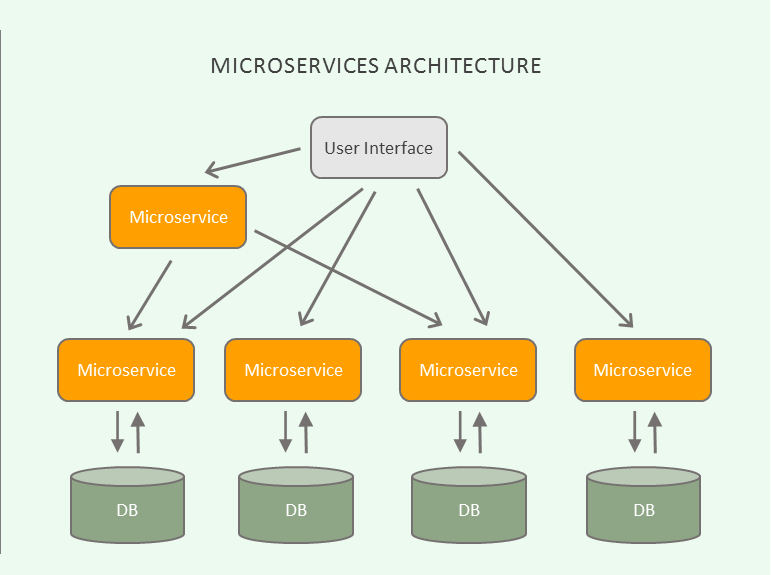
\includegraphics[width=0.95\textwidth]{Microservices.png}
\end{figure}

De service-interfaces zorgen voor een losse koppeling waardoor ze aangesproken kunnen worden met weinig of geen kennis van het onderliggend systeem. De services worden weergegeven met behulp van de standaard netwerkprotocollen zoals SOAP.

Ten opzichte van de standaard architecturen die SOA voorgingen (zoals de monoliet) bied het tal van voordelen:
\begin{itemize}
     \item \textbf{Flexibiliteit}: De mogelijkheid om componenten te hergebruiken zorgt ervoor dat een onderneming zich flexibeler kan opstellen en sneller kan reageren op marktsveranderingen. 
     \item \textbf{De mogelijkheid om legacy functionaliteit te integreren in nieuwe markten}: SOA biedt de mogelijkheid om functionaliteit van oude systemen te integreren naar nieuwe systemen.
     \item \textbf{Een betere connectie tussen IT en business}: In een SOA architectuur kunnen de services gedefinieerd worden als business termen. Hierdoor kunnen de analisten efficiënter werken en sneller de developers aanspreken. De scope van de services zijn ook makkelijker te definiëren.
\end{itemize} 

Veel experten beweren dat microservices de volgende stap is in de evolutie van SOA of dat het de correctie implementatie is van SOA. Er zijn tal van studies die deze twee architecturen vergelijken, maar voor dit onderzoek bespreken we enkel het verschil tussen de scope en de koppeling van de componenten. \textcite{Education2019}
\begin{figure}
    \caption{SOA vs Microservices}
    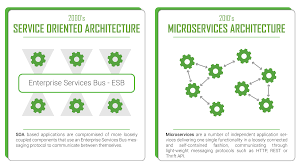
\includegraphics[width=1\textwidth]{SOAvsMicropng.png}
\end{figure}

SOA is een ondernemingsbreed concept. Het maakt het mogelijk om bestaande applicaties weer te geven via los gekoppelde interfaces, die elk verantwoordelijk zijn voor een bedrijfsfunctie, waardoor de applicaties een onderdeel vormen van een groot geheel. Vaak zijn deze componenten verbonden aan de hand van een integratie bus.

Microservices-architectuur is een concept met toepassingsbereik. Het splits de applicatie op in kleine onderdelen die onafhankelijk gewijzigd, geschaald en beheerd kunnen worden. Het definieert niet hoe applicaties met elkaar communiceren.


\subsection{Voordelen}
Om de impact te berekenen van de transformatie is het belangrijk dat de voordelen van een microservice architectuur gekend zijn. Om een standaard opsomming te vermijden en meer structuur te brengen in deze lijst, worden de voordelen onderverdeeld in 3 categorieen. In eerste instantie worden de voordelen besproken die horen bij het \underline{design} van mircoservices, vervolgens komt het gedeelte van de \underline{development} aan bod en tenslotte de \underline{deployment}.\\

\textbf{design}\\ 
Tijdens de design van een microservice-architectuur kunnen er al tal van voordelen genoteerd worden. Het ontwikkelen van deze architectuur zorgt ervoor dat men stil staat bij de scope van het project.\\ 
Een goed afgebakend project geeft een goed overzicht van de noden weer. Veel microservices maken gebruik van Cloud native computing wat meer flexibiliteit biedt. Microservices passen gedecentraliseerd beheer toe, wat betekent dat het development team de code kan ontwikkelen volgens hun individuele beheersplannen.\\ 
Het systeem zal ook zodanig ontwikkelt worden zodat wanneer een component uitvalt het systeem verder blijft werken. Deze eigenschap heet fouttolerantie. Een bijhorende patroon is het gebruik van een 'circuit breaker'. Deze service handelt fouten af die ontstaan bij het aanspreken van andere services.\\
Iedere service bevat zijn eigen database. Dit helpt mee aan de 'loosely coupled' strategie, veranderingen aan 1 database beïnvloedt de andere databases niet.\\
Services met gemeenschappelijke doeleinden kunnen gegroepeerd worden, hierdoor ontstaan 'lagen' van
componenten. Dit biedt de mogelijkheid om logica te hergebruiken en te isoleren.\\ \\
\textbf{development}\\ één van de grote voordelen van het ontwikkelen van microservices is dat developers zich kunnen concentreren op een service per keer. Ze hebben de vrijheid om te kiezen welke technologie ze willen gebruiken. Het is perfect mogelijk om 10 verschillende componenten in 10 verschillende technologieën te ontwikkelen. Natuurlijk moet er een consensus zijn over wat er wel of niet gebruikt mag worden. Bepaalde logica kan hergebruikt worden in meerdere services of een service kan verschillende componenten voeden waardoor veel werk herbruikbaar is. \\
Het ontwikkelen van integratie testen gaat ook sneller dankzij de kleinschalige componenten. Dependenties met andere services kunnen makkelijk opgevangen worden met Mocks.\\
Rollbacks zijn beperkter en hebben enkel impact op bepaalde services.\\ \\
\textbf{deployment}\\ Door gebruik te maken van microservices kan een onderneming kiezen om meerdere pipelines te gebruiken om een project in productie te plaatsen. Een pipeline per services is geen uitzondering. Hierdoor is de CI/CD van het project veel robuuster en zijn fouten sneller op te lossen.

\begin{figure}[!htb]
    \caption{pipelines monoliet versus microservices}
    \centering
    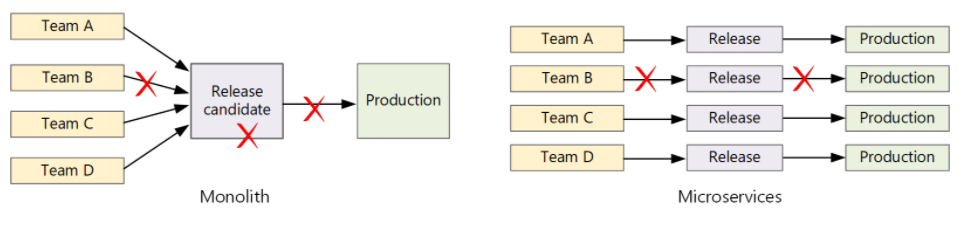
\includegraphics[width=0.9\textwidth]{PipelinesVS.png}    
\end{figure}

Het beheer van de code wordt ook een stuk eenvoudiger. Het uitvoeren van updates kan beter beheerd worden en geïsoleerd worden van componenten die de update niet nodig hebben.


\subsection{Pijnpunten}

Elke software architectuur heeft zijn uitdagingen of pijnpunten. Voor microservices is dit niet anders. Net zoals in sectie 1.1.2 verdelen we de nadelen op in 3 categorieën: \underline{design}, \underline{development} en \underline{deployment}.\\ \\

\textbf{design} \\De API dat geleverd wordt door een microservice wordt een soort contract tussen degelijke microservices en degenen die de API consumeren. Deze contracten zijn bindend en mogen niet geschonden worden. Dit heeft een negatieve impact op de versiebeheer van de API's geleverd door de microservices.\\    Toegangscontrole kan snel uit de hand lopen bij microservices. Elke service heeft zijn eigen noden en veel tools bieden enkel een gecentraliseerd beheer van accounts aan.\\    Microservices stellen meer API's bloot en distribueren authenticatie en toegangscontrole. Het oppervlak dat kwetsbaar is, is dus veel uitgebreider en dit is de belangrijkste reden waarom proliferatie van eindpunten significant wordt herkend als een pijnpunt door industriële onderzoekers en praktijkmensen.\\  \\
\textbf{development} \\ Als de opslagruimte gedeeld moet worden tussen de verschillende microservices, wordt het lastig om gegevensconsistentie te waarborgen. Dit is zeker het geval wanneer gevoelige data zoals contactgegevens gebruikt wordt over meerdere services.\\
Door de technische heterogeniteit kunnen verschillende technologieën gebruikt worden. Indien dit het geval is, dan is er een enorme reeks bekwame werknemers nodig om de grote heterogene gedistribueerde software te ondersteunen. Dit brengt een grote financiële kost met zich mee.\\
Het development team kan geografisch verspreid zijn. Componenten van de applicatie kunnen dus beheerd worden in verschillende landen. Dit vermoeilijkt de communicatie en vertraagt het ontwikkelingsproces.\\
De communicatie tussen de verschillende services gebeurd over een netwerk. Dit zorgt ervoor dat de services afhankelijk zijn van dit netwerk.\\ \\
\textbf{deployment} \\ Elke service zal zelf een logboek bijhouden, hierdoor moet er een extra service gecreëerd worden om alles logs te verzamelen in een overzicht.\\
De grootte en complexiteit van het implementatieproces kan voor sommige bedrijven een obstakel vormen.

\subsection{Toepassingen en design patterns}

Er zijn heel wat design patterns die gebruikt kunnen worden om de microservice architectuur te verwezelijken, zie figuur 1.3 . Om de scope van deze studie te beperken zullen we ze niet allemaal behandelen.\\ \\
\textbf{Aggregator Pattern}\\
Aggregator verwijst naar een website of programma dat gerelateerde gegevens verzamelt en weergeeft. In Microservices-patronen is Aggregator een basiswebpagina die verschillende services oproept om de vereiste informatie te verkrijgen of de correcte functionaliteit aan te bieden.\\
Het Aggregate Design Pattern is gebaseerd op het DRY-principe. Op basis van dit principe wordt de logica geabstraheerd in samengestelde microservices om daarna deze specifieke bedrijfslogica samen te voegen tot één service.
Bijvoorbeeld: twee services A en B kunnen afzonderlijk gelijktijdig geschaald worden door de gegevens aan de samengestelde microservice te verstrekken.

\begin{figure}[!htb]
    \caption{Aggragator Pattern}
    \centering
    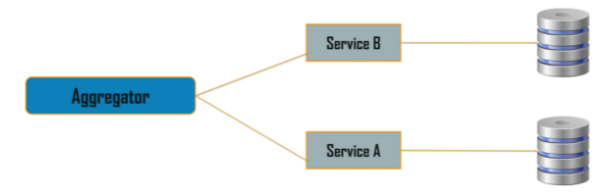
\includegraphics[width=1\textwidth]{Aggregator.png}
\end{figure}

\textbf{Strangler Pattern}\\
De strangler pattern is een manier om een legacy systeem stapsgewijs te migreren door bestaande functionaliteiten te vervangen door nieuwe applicaties en diensten in een gefaseerde aanpak. Over tijd zal het nieuwe systeem alle functionaliteit van het oude systeem bevatten en bijgevolg het systeem vervangen.

\begin{figure}[!htb]
    \caption{Straggler Pattern}
    \centering
    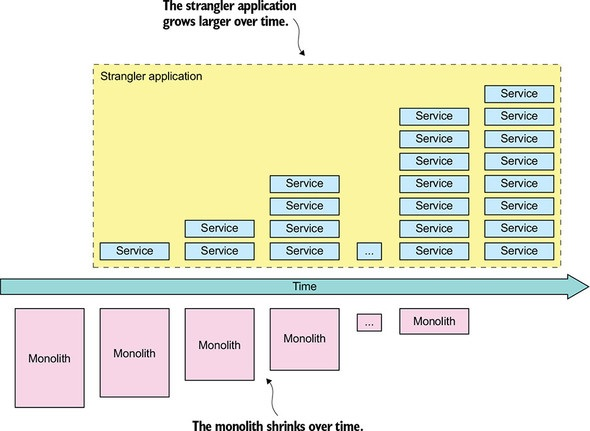
\includegraphics[height=8cm]{strangler.jpg}
\end{figure}

\textbf{Saga Pattern}
\\Een saga is een opeenvolging van lokale transacties. Elke lokale transactie werkt de database bij en publiceert een bericht of gebeurtenis om de volgende lokale transactie in de saga te activeren. Als een lokale transactie mislukt, voert de saga een rollback uit.\\
Dit patroon is toepasbaar wanneer elke service over zijn eigen database beschikt.

\begin{figure}[!htb]
    \caption{Saga Pattern}
    \centering
    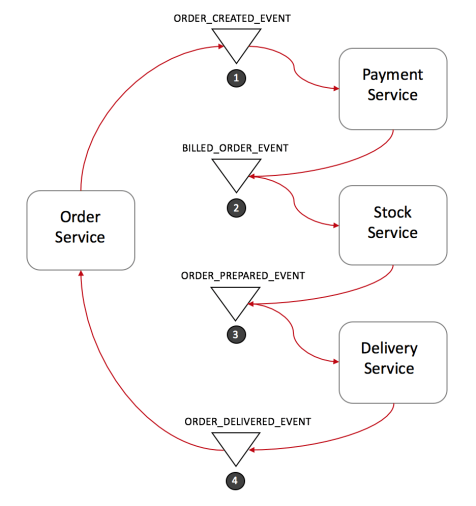
\includegraphics[height=10cm]{Saga.png}
\end{figure}

\textbf{Circuit Breaker}\\
Het idee achter de 'Circuit Breaker' is relatief eenvoudig. Net zoals een elektrische stroomonderbreker zal de service tijdelijk uitgeschakeld worden als er teveel fouten geregistreerd worden. In deze periode zullen alle pogingen om de service aan te roepen mislukken. Na deze periode zal de 'stroomonderbreker' een aantal verzoeken aanvaarden en controleren of de verzoeken slagen. Als deze controle succesvol is dat wordt de service hervat, zo niet dan blijft de 'stroomonderbreker' actief.
Er zijn drie toestanden: gesloten, half-open en open. In de gesloten toestand werkt alles zoals het hoort (zie afbeelding 1.6). 

\begin{figure}[!htb]
    \caption{Gesloten status}
    \centering
    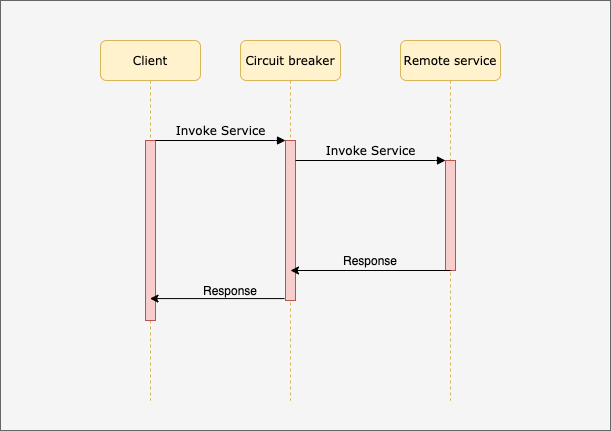
\includegraphics[height=10cm]{closed.png}
\end{figure}

Zodra het aantal storingen een vooraf bepaalde drempel overschrijdt, schakelt de stroomonderbreker uit en gaat deze in de open toestand(zie afbeelding 1.7).
\begin{figure}[!htb]
    \caption{Open status}
    \centering
    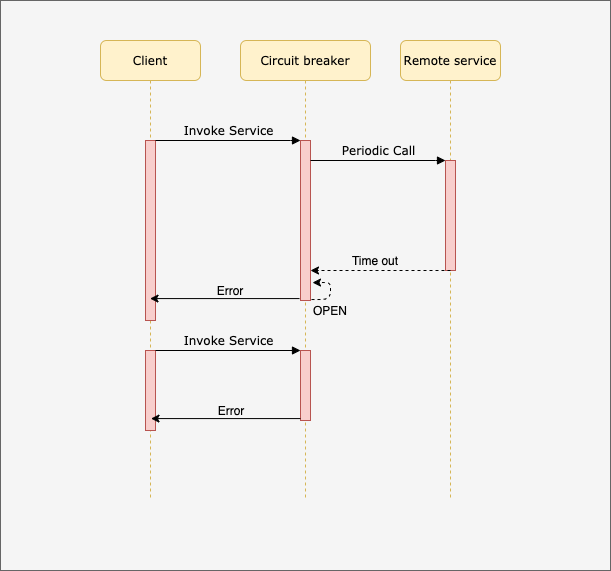
\includegraphics[height=11cm]{open.png}
\end{figure}

Na een bepaalde tijd schakelt het circuit over naar een half-open toestand (zie afbeelding 1.8) om te testen of het onderliggende probleem nog steeds bestaat. De 'stroomonderbreker' gebruikt een mechanisme om periodiek een proefoproep te doen naar de externe service om te controleren of deze is hersteld. Als de oproep naar de externe service mislukt, blijft de stroomonderbreker in de open toestand. Als de oproep succesvol terugkeert, schakelt het circuit over naar de gesloten status. De vermogensschakelaar stuurt dan alle externe oproepen naar de service terug met een fout tijdens de half-open toestand.

\begin{figure}[!htb]
    \caption{Half-open status}
    \centering
    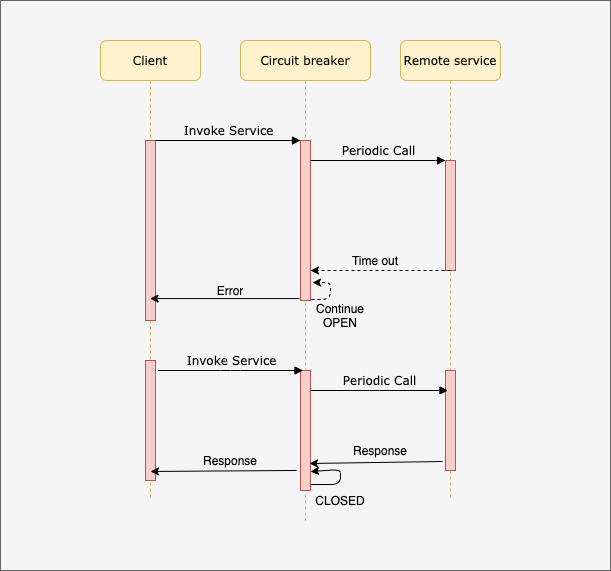
\includegraphics[height=10cm]{half-open.png}
\end{figure}

\textbf{Distributed Tracing}
Tracering is een fundamenteel proces in software-engineering, dat door programmeurs samen met andere vormen van registreren wordt gebruikt om informatie te verzamelen over het gedrag van een applicatie. Maar traditionele tracering stuit op problemen wanneer het wordt gebruikt om problemen op te lossen met applicaties die zijn gebouwd op een gedistribueerde softwarearchitectuur. Omdat microservices onafhankelijk schaalbaar zijn, is het gebruikelijk dat meerdere iteraties van een enkele service tegelijkertijd op verschillende servers, locaties en omgevingen worden uitgevoerd, waardoor een complex web ontstaat waar een verzoek doorheen moet. Deze verzoeken zijn bijna onmogelijk te volgen met traditionele technieken die zijn ontworpen voor een enkele servicetoepassing.
\\
Gedistribueerde traceringsoplossingen lossen dit probleem en tal van andere prestatieproblemen op, omdat het verzoeken via elke service of module kan volgen en een end-to-end narratief verslag van dat verzoek kan bieden. Analisten, SRE's, ontwikkelaars en anderen kunnen elke iteratie van een functie observeren, waardoor ze prestatiebewaking kunnen uitvoeren door te zien welke instantie van die functie ervoor zorgt dat de app vertraagt of faalt, en hoe ze dit kunnen oplossen. (zie figuur 1.9)

\begin{figure}[!htb]
    \caption{Distributed Tracing}
    \centering
    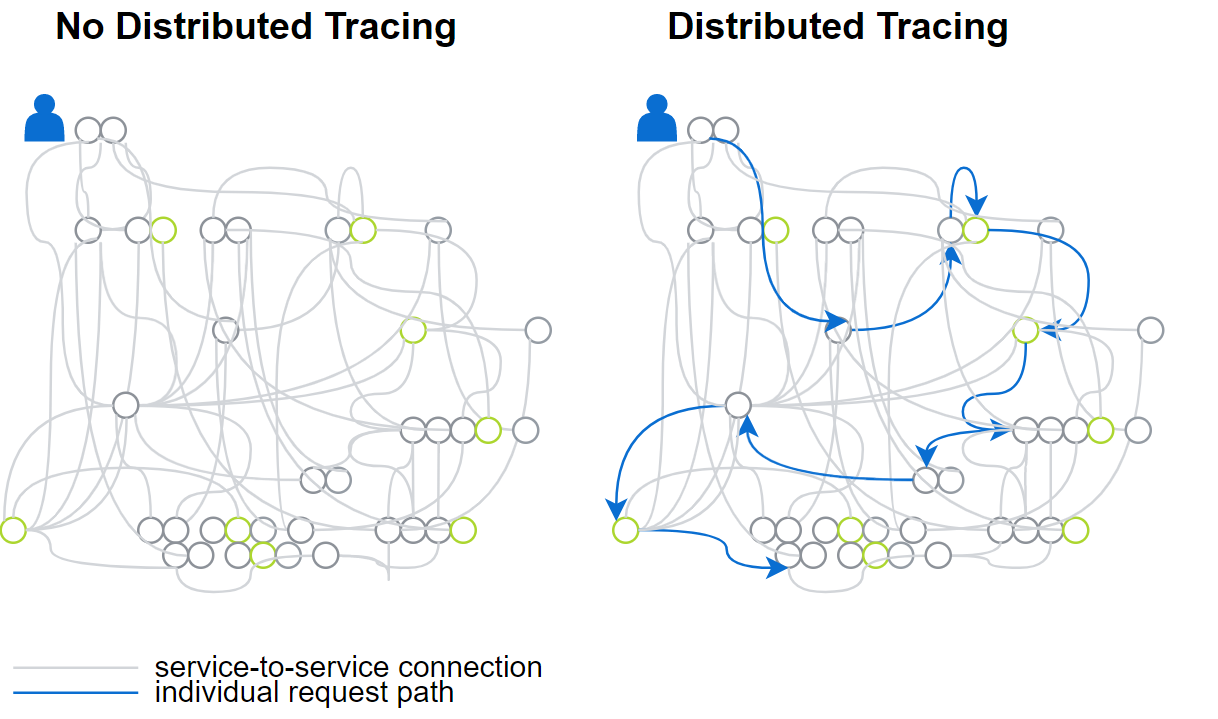
\includegraphics[height=10cm]{DistributedTracing.png}
\end{figure}
\begin{figure}[!htb]
    \caption{Overzicht Design Patterns}
    \centering
    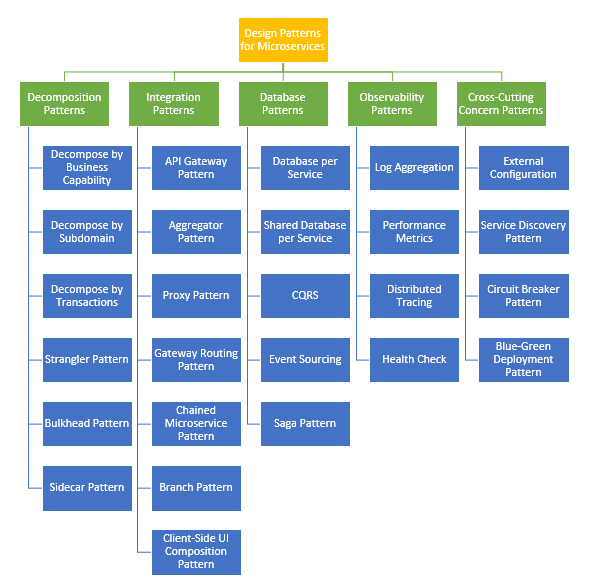
\includegraphics[height=11cm]{DesignPatterns.png}
\end{figure}
\newpage
\subsection{Micro Frontends}
Een volgende stap is om het concept van micro services toe te passen op de frontend. De huidige trend in web ontwikkeling zijn single page applicaties. De bekendste en meeste gebruikte SPA frameworks zijn React, Angular en Vue. In vele gevallen wordt de frontend onderhouden door één afzonderlijk team. Hierdoor groeit de frontend laag geleidelijk aan in een groot project, ook wel een frontend monoliet genoemd.\\\\
Het idee achter de Micro frontends is om de website op te delen op basis van features en met behulp van compositie de verschillende delen samen te brengen in een werkende website. In theorie worden de features onderhouden door onafhankelijke teams. Elk team is verantwoordelijk voor zijn feature. De teams hebben een bepaald doel en dat doel is meestal gekoppeld aan een business requirement. Het team ontwikkeld  alles zelfstandig, vanaf het moment de data opgehaald wordt uit de database  tot en met de user interface. In het verleden werden dergelijke benaderingen ‘frontend integratie voor verticale systemen’ genoemd. Micro frontends is bij uitstek de elegantere benaming.

De kernideeën achter Micro frontends:
\begin{itemize}
    \item \textbf{Team code is geïsoleerd} \\
          Elk team heeft zijn eigen stack en pipeline waar hun code gebouwd wordt. Afhankelijkheden op andere teams worden vermeden.
    \item \textbf{Elke team bepaalt hun eigen technologie} \\
          De teams hebben de vrijheid om de technologie te kiezen die zij wensen te gebruiken. Zonder af te stemmen met andere teams. 
    \item \textbf{Teamvoorvoegsels instellen}\\
          Op plaatsen waar het niet mogelijk is om code te isoleren, moet het duidelijk zijn welk team eigenaar is van de niet geïsoleerde code. Dit kan gerealiseerd worden met naamgevingsconventies.  
    \item \textbf{Verkies browserfuncties boven aangepaste API’s}\\
          In eerste instantie worden browserfuncties gebruikt om te communiceren. Als deze functionaliteit ontoereikend is, kan er voor een aangepaste API geopteerd worden. 
    \item \textbf{Bouw een veerkrachtige website}
          Elke feature moet zijn nut hebben. Als dit niet het geval is, moet de feature verwijderd worden of geabsorbeerd worden in een ander team.\\
\end{itemize}
\subsection{Mono- en polyrepo}
Wanneer alle code in één dezelfde repository bijgehouden wordt, spreken we over een monorepo. De apps zijn dan onderverdeeld in verschillende subfolders. Deze structuur komt in veel projecten voor. Code in deze structuur heeft meestal één pipeline voor de implementatie. Dit zorgt voor een eenvoudige onderhoud, maar een enkele bug kan het hele proces vertragen.\\ 
Wanneer de code opgedeeld wordt in verschillende repositories, spreken we over een polyrepo. Een project is dan verspreid over meerdere bronnen. Dit heeft tal van voordelen maar brengt ook wat nadelen met zich mee.\\
Bedrijven die gebruik maken van microservices delen snel hun code op in verschillende repositories (polyrepos).  De teams ontwikkelen hun services onafhankelijk van elkaar en bij gevolg gebruiken ze dus hun eigen repo. De voordelen van deze structuur zijn duidelijk. Een klein team kan snel en zonder restricties hun eigen code in productie plaatsen.\\  
Het nadeel is dat alle kennis verspreid is over verschillende repos, in het slechtste geval kom je op een punt waarbij niemand meer weet hoe het volledige systeem opgebouwd en geïmplementeerd wordt. \\
\\
Het gebruik van een enkele repo (monorepo) heeft enkele voordelen:
\begin{itemize}
    \item \textbf{Beter overzicht}\\
        Als een service gebruikt maakt van een andere service, zal het makkelijker zijn om te zien wat er precies in de code gebeurd. Bugs kunnen hierdoor sneller toegewezen worden aan een team.
    \item \textbf{Hergebruik van code}\\
        Er zal altijd gemeenschappelijke code zijn tussen verschillende services. Als het team kiest om deze code niet te dupliceren, is het makkelijker om in een monorepo de code te hergebruiken. Dit gaat wel in tegen het principe dat elke service onafhankelijk en geïsoleerd moet zijn.
    \item \textbf{Verbeterede samenwerking}\\
        Een enkele repository verwijdert de barrière tussen teams. Het zorgt voor meer toegankelijkheid. 
    \item \textbf{Standaardisatie}\\
        Het is eenvoudiger om code te standaardiseren en om een beleid te hanteren. Dit gaat natuurlijk weer in tegen de principes van mircoservices.
    \item \textbf{Refactoring}\\
        Het is minder werk om code structuren aan te passen in een enkele repository dan code die verspreidt is over meerder repositories.
    \item \textbf{Kennis}\\
        Alle logica is terug te vinden in enkele repo, hierdoor is er minder verlies van kennis over de jaren heen.
\end{itemize}
Een monorepo brengt ook wat uitdagingen met zich mee. Simpele aanpassingen in de code kan een grote impact hebben op andere componenten. Het implementatie proces is ingewikkelder en kan bij foute implementatie heel wat vertraging opleveren.\\ 
Beide strategieën hebben hun voor- en nadelen, er is geen winnaar. Het team kiest welk systeem het best aan hun noden voldoet.

\newpage
\section{Monolithische architectuur}
Een monololitische architectuur betekent dat alles uit één stuk samengesteld is. De Monololitisch applicatie beschrijft een softwareapplicatie waarin verschillende componenten worden gecombineerd tot een enkel programma vanaf een enkel platform. De volgende componenten kunnen voorkomen:
\begin{itemize}
    \item Authorisatie
    \item Presentatie
    \item Business logica
    \item Database laag
    \item applicatie integratie
    \item notificatie module
\end{itemize}
\begin{figure}[!htb]
    \caption{Monolithische architectuur}
    \centering
    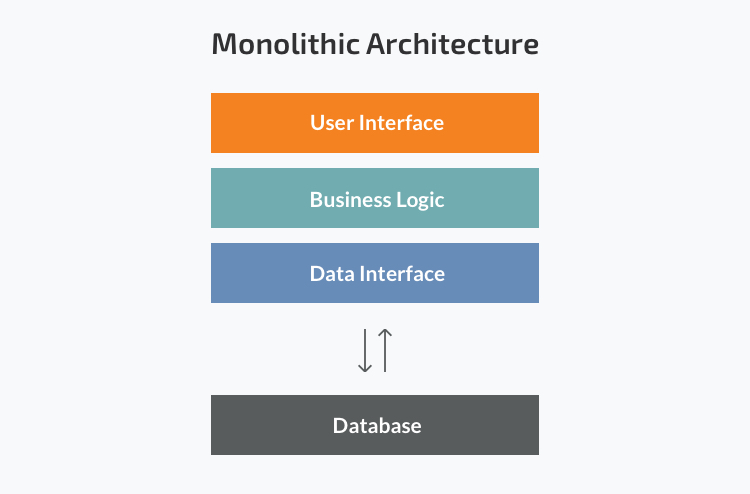
\includegraphics[width=1\textwidth]{Monoliet.png}
\end{figure}
Deze achitectuurvorm biedt de meeste voordelen bij kleinschalige projecten of systemen. Mits alles één geheel vormt, is een dergelijke applicatie makkelijk te ontwikkelen en ligt de progressiesnelheid relatief hoog. Hoe groter het project hoe meer problemen zich voordoen bij monolithische systemen. De codekwaliteit zal snel dalen als er meer duplicate code zal onstaan. Nieuwe features zullen trager ontwikkeld worden. Bugs zullen minder snel opgespoord worden. Een bijkomend probleem is dat nieuwe developers tijd zullen nodig hebben om in het project mee te stappen omdat de kennis hoofdzakelijk bij de originele ontwikkelaars zit. \\
De applicatie is makkelijk om in productie te plaatsen. Het nadeel is dat bij elke update het volledige deployprocess uitgevoerd wordt. Hierdoor is het onmogelijk om CI/CD te implementeren en wordt er meestal met vast deploy moment gewerkt. Als de update mislukt moet het volledige systeem terug gedraaid worden.\\
De applicatie zal hoogstens één technologie bevatten. Hierdoor is het systeem volledig afhankelijk van die ene technologie. Dit zorgt ervoor dat de onderneming minder snel op marktsverandering kan inspelen.\\
Het systeem in productie kan enkel horizontaal geschaald worden. Dit beperkt de opties die mogelijk zijn om extra resources toe te voegen. 

\end{document}